\documentclass[11pt]{article}
\usepackage{amsgen,amsmath,amstext,amsbsy,amsopn,amssymb}
%\usepackage[dvips]{graphicx,color}
\usepackage{graphicx,color}
\usepackage{graphicx,color,bm}
\usepackage{epsfig}
\usepackage{enumerate}
\usepackage{float}
%\setlength{\oddsidemargin}{0.1 in} \setlength{\evensidemargin}{-0.1
%in} \setlength{\topmargin}{-0.6 in} \setlength{\textwidth}{6.5 in}
%\setlength{\textheight}{8.5 in} \setlength{\headsep}{0.75 in}
%\setlength{\parindent}{0 in} \setlength{\parskip}{0.1 in}

\textwidth 6.3in \textheight 8.8in \topmargin -0.5truein
\oddsidemargin .15truein
\parskip .1in
\renewcommand{\baselinestretch}{1.53}  % double spaced


\newcommand{\homework}[6]{
	\pagestyle{myheadings}
	\thispagestyle{plain}
	\newpage
	\setcounter{page}{1}
	\noindent
	\begin{center}
		\framebox{
			\vbox{\vspace{2mm}
				\hbox to 6.28in { {\bf Math531:~Regression - I  \hfill} }
				\vspace{6mm}
				\hbox to 6.28in { {\Large \hfill #1 (#2)  \hfill} }
				\vspace{6mm}
				\hbox to 6.28in { {\it Instructor: #3 \hfill} }
				\hbox to 6.28in { {\it Office hours: #4  \hfill #6}}
				\vspace{2mm}}
		}
	\end{center}
	\markboth{#1}{#1}
	\vspace*{4mm}
}

% ----------------------- MATH -------------------------
\def\av{\boldsymbol a}
\def\bv{\boldsymbol b}
\def\cv{\boldsymbol c}
\def\dv{\boldsymbol d}
\def\ev{\boldsymbol e}
\def\fv{\boldsymbol f}
\def\gv{\boldsymbol g}
\def\hv{\boldsymbol h}
\def\iv{\boldsymbol i}
\def\gv{\boldsymbol j}
\def\kv{\boldsymbol k}
\def\lv{\boldsymbol l}
\def\mv{\boldsymbol m}
\def\nv{\boldsymbol n}
\def\ov{\boldsymbol o}
\def\pv{\boldsymbol p}
\def\qv{\boldsymbol q}
\def\rv{\boldsymbol r}
\def\sv{\boldsymbol s}
\def\tv{\boldsymbol t}
\def\uv{\boldsymbol u}
\def\vv{\boldsymbol v}
\def\wv{\boldsymbol w}
\def\xv{\boldsymbol x}
\def\yv{\boldsymbol y}
\def\zv{\boldsymbol z}
\def\Av{\boldsymbol A}
\def\Bv{\boldsymbol B}
\def\Cv{\boldsymbol C}
\def\Dv{\boldsymbol D}
\def\Ev{\boldsymbol E}
\def\Fv{\boldsymbol F}
\def\Gv{\boldsymbol G}
\def\Hv{\boldsymbol H}
\def\Iv{\boldsymbol I}
\def\Gv{\boldsymbol J}
\def\Kv{\boldsymbol K}
\def\Lv{\boldsymbol L}
\def\Mv{\boldsymbol M}
\def\Nv{\boldsymbol N}
\def\Ov{\boldsymbol O}
\def\Pv{\boldsymbol P}
\def\Qv{\boldsymbol Q}
\def\Rv{\boldsymbol R}
\def\Sv{\boldsymbol S}
\def\Tv{\boldsymbol T}
\def\Uv{\boldsymbol U}
\def\Vv{\boldsymbol V}
\def\Wv{\boldsymbol W}
\def\Xv{\boldsymbol X}
\def\Yv{\boldsymbol Y}
\def\Zv{\boldsymbol Z}
\def\Abf{\mathbf A}
\def\Bbf{\mathbf B}
\def\Cbf{\mathbf C}
\def\Dbf{\mathbf D}
\def\Ebf{\mathbf E}
\def\Fbf{\mathbf F}
\def\Gbf{\mathbf G}
\def\Hbf{\mathbf H}
\def\Ibf{\mathbf I}
\def\Gbf{\mathbf J}
\def\Kbf{\mathbf K}
\def\Lbf{\mathbf L}
\def\Mbf{\mathbf M}
\def\Nbf{\mathbf N}
\def\Obf{\mathbf O}
\def\Pbf{\mathbf P}
\def\Qbf{\mathbf Q}
\def\Rbf{\mathbf R}
\def\Sbf{\mathbf S}
\def\Tbf{\mathbf T}
\def\Ubf{\mathbf U}
\def\Vbf{\mathbf V}
\def\Wbf{\mathbf W}
\def\Xbf{\mathbf X}
\def\Ybf{\mathbf Y}
\def\Zbf{\mathbf Z}
\def\Am{\mathrm A}
\def\Bm{\mathrm B}
\def\Cm{\mathrm C}
\def\Dm{\mathrm D}
\def\Em{\mathrm E}
\def\Fm{\mathrm F}
\def\Gm{\mathrm G}
\def\Hm{\mathrm H}
\def\Im{\mathrm I}
\def\Gm{\mathrm J}
\def\Km{\mathrm K}
\def\Lm{\mathrm L}
\def\Mm{\mathrm M}
\def\Nm{\mathrm N}
\def\Om{\mathrm O}
\def\Pm{\mathrm P}
\def\Qm{\mathrm Q}
\def\Rm{\mathrm R}
\def\Sm{\mathrm S}
\def\Tm{\mathrm T}
\def\Um{\mathrm U}
\def\mv{\mathrm V}
\def\Wm{\mathrm W}
\def\Xm{\mathrm X}
\def\Ym{\mathrm Y}
\def\Zm{\mathrm Z}
\newcommand{\Ac}{\mathcal{A}}
\newcommand{\Bc}{\mathcal{B}}
\newcommand{\Cc}{\mathcal{C}}
\newcommand{\Dc}{\mathcal{D}}
\newcommand{\Ec}{\mathcal{E}}
\newcommand{\Fc}{\mathcal{F}}
\newcommand{\Gc}{\mathcal{G}}
\newcommand{\Hc}{\mathcal{H}}
\newcommand{\Ic}{\mathcal{I}}
\newcommand{\Jc}{\mathcal{J}}
\newcommand{\Kc}{\mathcal{K}}
\newcommand{\Lc}{\mathcal{L}}
\newcommand{\Mc}{\mathcal{M}}
\newcommand{\Nc}{\mathcal{N}}
\newcommand{\Oc}{\mathcal{O}}
\newcommand{\Pc}{\mathcal{P}}
\newcommand{\Qc}{\mathcal{Q}}
\newcommand{\Rc}{\mathcal{R}}
\newcommand{\Sc}{\mathcal{S}}
\newcommand{\Tc}{\mathcal{T}}
\newcommand{\Uc}{\mathcal{U}}
\newcommand{\Vc}{\mathcal{V}}
\newcommand{\Wc}{\mathcal{W}}
\newcommand{\Xc}{\mathcal{X}}
\newcommand{\Yc}{\mathcal{Y}}
\newcommand{\Zc}{\mathcal{Z}}
\newcommand{\alphav}{\mbox{\boldmath{$\alpha$}}}
\newcommand{\betav}{\mbox{\boldmath{$\beta$}}}
\newcommand{\gammav}{\mbox{\boldmath{$\gamma$}}}
\newcommand{\deltav}{\mbox{\boldmath{$\delta$}}}
\newcommand{\epsilonv}{\mbox{\boldmath{$\epsilon$}}}
\newcommand{\zetav}{\mbox{\boldmath$\zeta$}}
\newcommand{\etav}{\mbox{\boldmath{$\eta$}}}
\newcommand{\iotav}{\mbox{\boldmath{$\iota$}}}
\newcommand{\kappav}{\mbox{\boldmath{$\kappa$}}}
\newcommand{\lambdav}{\mbox{\boldmath{$\lambda$}}}
\newcommand{\muv}{\mbox{\boldmath{$\mu$}}}
\newcommand{\nuv}{\mbox{\boldmath{$\nu$}}}
\newcommand{\xiv}{\mbox{\boldmath{$\xi$}}}
\newcommand{\omicronv}{\mbox{\boldmath{$\omicron$}}}
\newcommand{\piv}{\mbox{\boldmath{$\pi$}}}
\newcommand{\rhov}{\mbox{\boldmath{$\rho$}}}
\newcommand{\sigmav}{\mbox{\boldmath{$\sigma$}}}
\newcommand{\tauv}{\mbox{\boldmath{$\tau$}}}
\newcommand{\upsilonv}{\mbox{\boldmath{$\upsilon$}}}
\newcommand{\phiv}{\mbox{\boldmath{$\phi$}}}
\newcommand{\varphiv}{\mbox{\boldmath{$\varphi$}}}
\newcommand{\chiv}{\mbox{\boldmath{$\chi$}}}
\newcommand{\psiv}{\mbox{\boldmath{$\psi$}}}
\newcommand{\omegav}{\mbox{\boldmath{$\omega$}}}
\newcommand{\Sigmav}{\mbox{\boldmath{$\Sigma$}}}
\newcommand{\Lambdav}{\mbox{\boldmath{$\Lambda$}}}
\newcommand{\Deltav}{\mbox{\boldmath{$\Delta$}}}
\newcommand{\Omegav}{\mbox{\boldmath{$\Omega$}}}
\newcommand{\varepsilonv}{\mbox{\boldmath{$\varepsilon$}}}

\newcommand{\eps}{\varepsilon}
\newcommand{\epsv}{\mbox{\boldmath{$\varepsilon$}}}

\def\1v{\mathbf 1}
\def\0v{\mathbf 0}
\def\Id{\mathbf I} % identity matrix
\newcommand{\ind}[1]{\mathbbm{1}_{\left[ {#1} \right] }}
\newcommand{\Ind}[1]{\mathbbm{1}_{\left\{ {#1} \right\} }}
\newcommand\indep{\protect\mathpalette{\protect\independenT}{\perp}}\def\independenT#1#2{\mathrel{\rlap{$#1#2$}\mkern2mu{#1#2}}}
\newcommand{\QED}{\begin{flushright} {\bf QED} \end{flushright}}
\newcommand{\R}{\mathbb R}
\newcommand{\Real}{\mathbb R}
\newcommand{\C}{\mathbb C}
\newcommand{\E}{\mathbb E}
\newcommand{\sgn}{\mathop{\mathrm{sign}}}
\def\Pr{\mathrm P}
\def\pr{\mathrm P}
\newcommand{\Var}{\mathop{\rm Var}}
\newcommand{\var}{\mathop{\rm Var}}
\newcommand{\Cov}{\mathop{\rm Cov}}
\newcommand{\cov}{\mathop{\rm Cov}}
\newcommand{\Corr}{\mathop{\rm Corr}}
\newcommand{\ang}{\mathop{\rm Angle}}
\newcommand{\tr}{\mathop{\rm trace}}
\newcommand{\proj}{\mathop{\rm Proj}}
\newcommand{\rank}{\mathop{\rm rank}}

\newcommand{\diag}{\mathop{\rm diag}}
\newcommand{\Diag}{\mathop{\rm diag}}
\newcommand{\sk}{\vspace{0.5cm}}
\newcommand{\ds}{\displaystyle}
\newcommand{\mb}{\mbox}
\newcommand{\wh}{\widehat}
\newcommand{\argmin}{\operatornamewithlimits{argmin}}
\newcommand{\argmax}{\operatornamewithlimits{argmax}}

\newcommand{\norm}[1]{\|#1\|}
\newcommand{\abs}[1]{\left\vert#1\right\vert}
\newcommand{\set}[1]{\left\{#1\right\}}

\newcommand{\To}{\longrightarrow}

\def\equalLaw{\stackrel{\mathcal{L}}{=}}
\def\equallaw{\stackrel{\mathcal{L}}{=}}

\def\half{\frac{1}{2}}

\usepackage{caption}

\begin{document}

\begin{title}
	{\Large\bf Homework 5, Math 455: Due Monday, 03/26/2018}
\end{title}

\author{\bf Alexander Van Roijen}

\maketitle
{\bf Instructions}:  The homework assignment editing this \LaTeX\ document.  Download the \LaTeX\ source from the class web page and study
it to learn more about \LaTeX.  Replace the text with appropriate information.  Run ``pdflatex'' on this document.

You will submit this assignment in two parts:
\begin{enumerate}
\item Print out the PDF file and bring it to class, and
\item Send an e-mail to:
\begin{center}
gang@math.binghamton.edu
\end{center}
\emph{before class} on the due date with two attachments:
\begin{itemize}
\item The \LaTeX\ source file, and
\item The generated PDF document.
\end{itemize}
\end{enumerate}
\newpage
Please complete the following:
\begin{enumerate}
\item  Finish 6.1, 6.2,6.3,6.4, 6.5, 6.6 from the textbook.  Submit your
answers for {\color{red}ALL} questions.\\
NOTE: ALL graphs and images that are not deemed meaningful will not be included
\end{enumerate}
\begin{enumerate}
	\item
	We first check the constant variance assumption. At a glance, it seems to be fine, however you may be able to argue it has a non linear pattern.
	\begin{figure}[H]
		\centering
		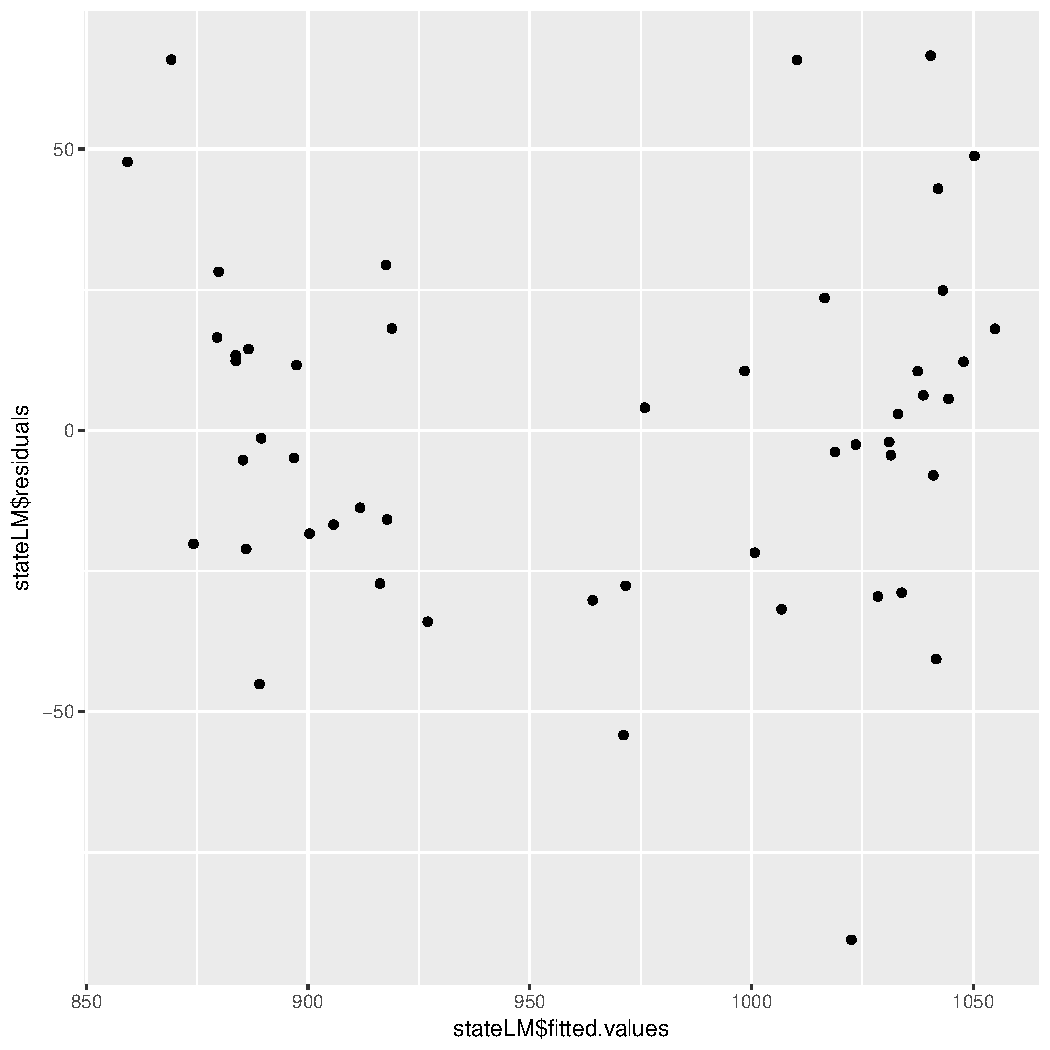
\includegraphics[width=10cm,height=10cm]{satcv.pdf}
		\caption[satcv]{constant variance check on sat data}
		\label{CV check on SAT}
	\end{figure}
	we then check our normality assumption using a qqplot. looks good still.\\
	We check for large leverage points and find the following\\
	\begin{verbatim}
		> hats[which.max(abs(hats))]
		Utah 
		0.2921128 
	\end{verbatim}
	further, looking at the following halfnormal graph for cooks distance, we again see Utah
	\begin{figure}[H]
		\centering
		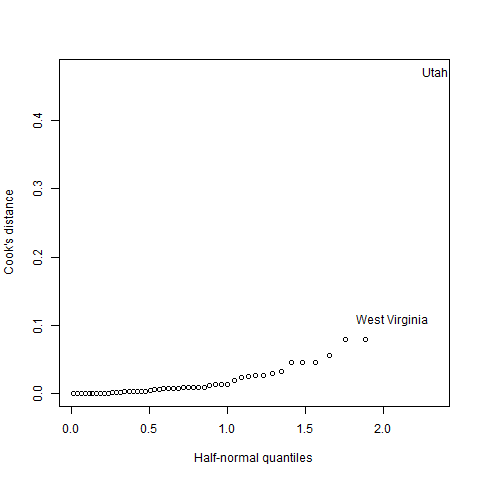
\includegraphics[width=15cm,height=15cm]{satCD.png}
		\caption[satCD]{cooks distances from sat data}
		\label{cooks distanced sat}
	\end{figure}
	Taking a closer look:
	\begin{verbatim}
		> sat[c('Utah'),]
		expend ratio salary takers verbal math total
		Utah  3.656  24.3 29.082      4    513  563  1076
	\end{verbatim}
	We have a very high total, but a very low expenditure and a very low percentage of takers. This is giving a really high total for a state with very few takers. This outlier throws off our model quite a bit. Removing it, we see the following difference in model values and performance
	\begin{verbatim}
		> stateLM2 = lm(total~expend+salary+ratio+takers,subset = satCook < max(satCook),sat)
		> summary(stateLM)
		
		Call:
		lm(formula = y ~ expend + salary + ratio + takers, data = sat)
		
		Residuals:
		Min      1Q  Median      3Q     Max 
		-90.531 -20.855  -1.746  15.979  66.571 
		
		Coefficients:
		Estimate Std. Error t value Pr(>|t|)    
		(Intercept) 1045.9715    52.8698  19.784  < 2e-16 ***
		expend         4.4626    10.5465   0.423    0.674    
		salary         1.6379     2.3872   0.686    0.496    
		ratio         -3.6242     3.2154  -1.127    0.266    
		takers        -2.9045     0.2313 -12.559 2.61e-16 ***
		---
		Signif. codes:  0 ‘***’ 0.001 ‘**’ 0.01 ‘*’ 0.05 ‘.’ 0.1 ‘ ’ 1
		
		Residual standard error: 32.7 on 45 degrees of freedom
		Multiple R-squared:  0.8246,	Adjusted R-squared:  0.809 
		F-statistic: 52.88 on 4 and 45 DF,  p-value: < 2.2e-16
		
		> summary(stateLM2)
		
		Call:
		lm(formula = total ~ expend + salary + ratio + takers, data = sat, 
		subset = satCook < max(satCook))
		
		Residuals:
		Min      1Q  Median      3Q     Max 
		-92.118 -18.402   1.808  14.890  67.669 
		
		Coefficients:
		Estimate Std. Error t value Pr(>|t|)    
		(Intercept) 1093.8460    53.4226  20.475   <2e-16 ***
		expend        -0.9427    10.1922  -0.092    0.927    
		salary         3.0964     2.3283   1.330    0.190    
		ratio         -7.6391     3.4279  -2.229    0.031 *  
		takers        -2.9308     0.2188 -13.397   <2e-16 ***
		---
		Signif. codes:  0 ‘***’ 0.001 ‘**’ 0.01 ‘*’ 0.05 ‘.’ 0.1 ‘ ’ 1
		
		Residual standard error: 30.9 on 44 degrees of freedom
		Multiple R-squared:  0.8396,	Adjusted R-squared:  0.825 
		F-statistic: 57.58 on 4 and 44 DF,  p-value: < 2.2e-16
	\end{verbatim}
	We see that ratio becomes insignificant if we remove utah from this data set. We also see an improved R squared value.
	\\
	I personally would reconsider removing utah, as I find some more information from utah might help quite a bit.
	\\
	Note: summaries of data sets will be deprecated to key information from this point forward. In detail summaries can be found in the R code.
	\item
	looking at our teen gambling data set, we immediately see that there is a non constant variance
	\begin{figure}[H]
		\centering
		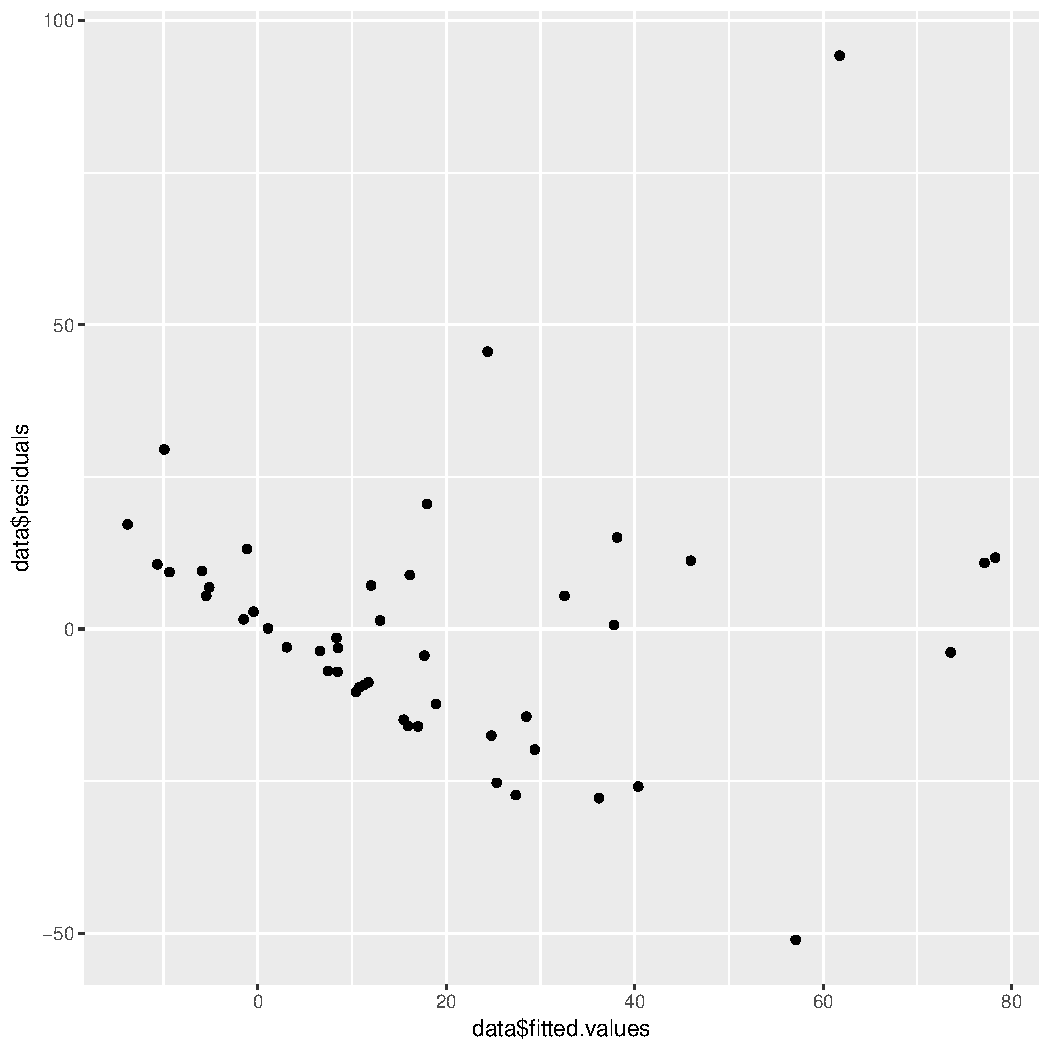
\includegraphics[width=10cm,height=10cm]{teengambcv.pdf}
		\caption[teengambcv]{constant variance check on teen gamb data}
		\label{CV check on teen gamb}
	\end{figure}
	we try to improve it by some transformations, but it still isnt quite satisfactory. The best is upon taking the square root of the response variable.
	\begin{figure}[H]
		\centering
		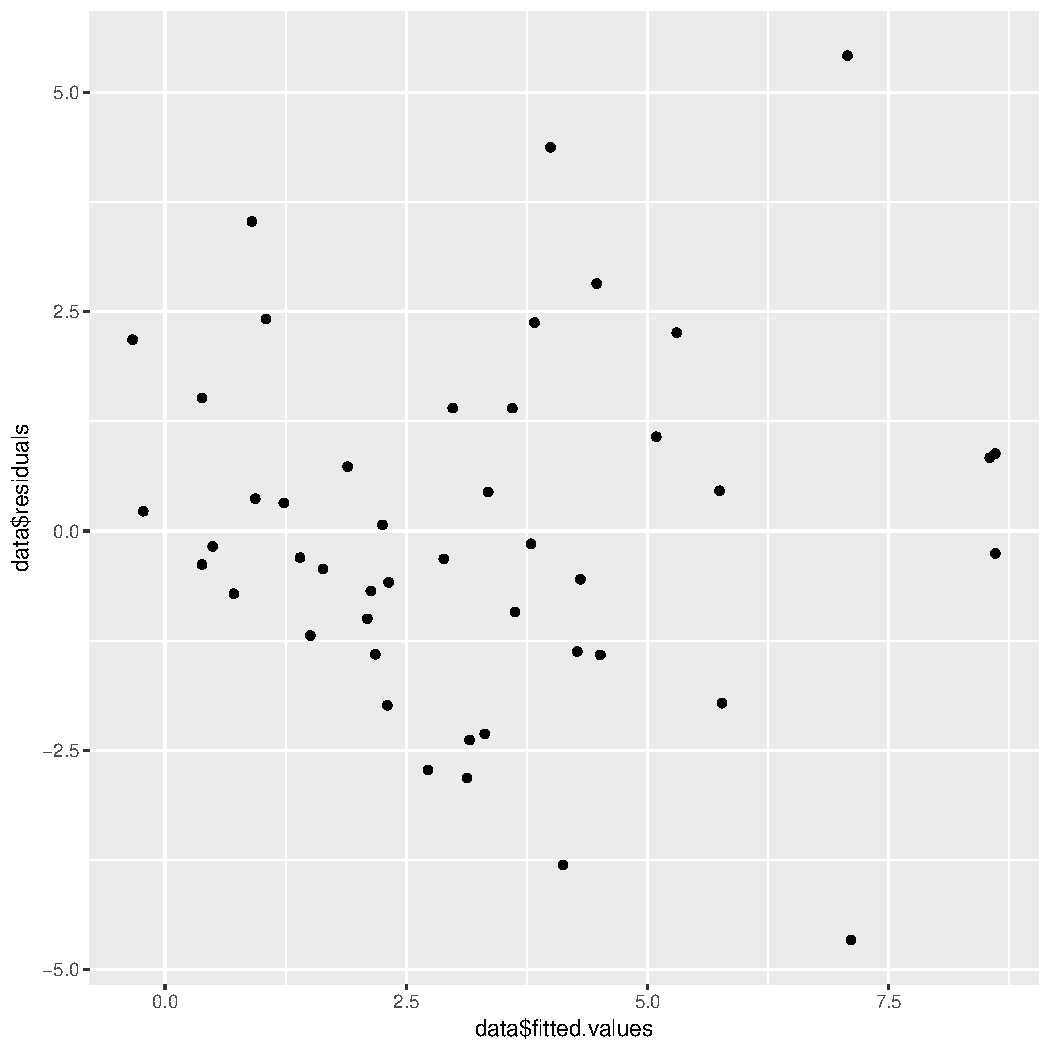
\includegraphics[width=6cm,height=6cm]{teengambcv2.pdf}
		\caption[teengambcv]{constant variance check on teen gamb data}
		\label{CV check on teen gamb}
	\end{figure}
	However, we continue to identify any outliers and come across one instance, row 24, we have a very high cooks distance
	\begin{figure}[H]
		\centering
		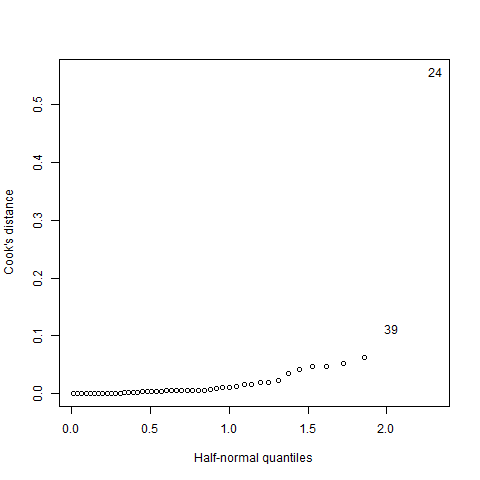
\includegraphics[width=8cm,height=8cm]{teengambCD.png}
		\caption[teengambCD]{cooks distances from teen gamb data}
		\label{CD check on teen gamb}
	\end{figure}
	we look at row 24, see it has a very high gamble value, and we then retry our model with this particular data point removed.
	\begin{verbatim}
		> teengamb[24,]
		sex status income verbal gamble
		24   0     27     10      4    156
		
		> tmodel2 = lm(gamble~.,subset = weirdo< max(weirdo),teengamb)
		> summary(tmodel)
		
		Coefficients:
		Estimate Std. Error t value Pr(>|t|)    
		(Intercept)  22.55565   17.19680   1.312   0.1968    
		sex         -22.11833    8.21111  -2.694   0.0101 *  
		status        0.05223    0.28111   0.186   0.8535    
		income        4.96198    1.02539   4.839 1.79e-05 ***
		verbal       -2.95949    2.17215  -1.362   0.1803    
		
		Residual standard error: 22.69 on 42 degrees of freedom
		Multiple R-squared:  0.5267,	Adjusted R-squared:  0.4816 
		F-statistic: 11.69 on 4 and 42 DF,  p-value: 1.815e-06
		
		> summary(tmodel2)
		
		Coefficients:
		Estimate Std. Error t value Pr(>|t|)    
		(Intercept)   7.6306    12.9251   0.590   0.5582    
		sex         -16.2986     6.1335  -2.657   0.0112 *  
		status        0.1739     0.2083   0.835   0.4088    
		income        4.3312     0.7636   5.672 1.26e-06 ***
		verbal       -1.8019     1.6137  -1.117   0.2707    
		
		Residual standard error: 16.74 on 41 degrees of freedom
		Multiple R-squared:  0.5682,	Adjusted R-squared:  0.526 
		F-statistic: 13.49 on 4 and 41 DF,  p-value: 4.225e-07
	\end{verbatim}
	again, we see adjusted p values, coefficient values, and R squared.
	\item
	Looking at the prostate data set, everything looks good in regards to structure, and normality assumptions. When we look at cooks distances however, we find quite a few values having abnormally high values.
	\begin{figure}[H]
		\centering
		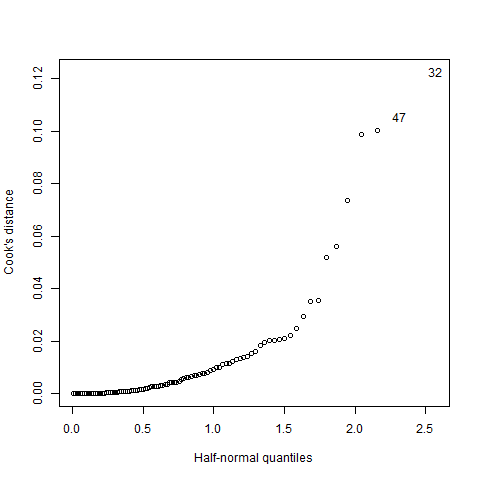
\includegraphics[width=8cm,height=8cm]{prostateCD.png}
		\caption[prostateCD]{cooks distances from prostate data}
		\label{CD check on teen gamb}
	\end{figure}
	we remove the highest point, 32, and see the below changes in our models. 
	\begin{verbatim}
		> summary(pmodel)

		Coefficients:
		Estimate Std. Error t value Pr(>|t|)    
		(Intercept)  0.669337   1.296387   0.516  0.60693    
		lcavol       0.587022   0.087920   6.677 2.11e-09 ***
		lweight      0.454467   0.170012   2.673  0.00896 ** 
		age         -0.019637   0.011173  -1.758  0.08229 .  
		lbph         0.107054   0.058449   1.832  0.07040 .  
		svi          0.766157   0.244309   3.136  0.00233 ** 
		lcp         -0.105474   0.091013  -1.159  0.24964    
		gleason      0.045142   0.157465   0.287  0.77503    
		pgg45        0.004525   0.004421   1.024  0.30886    
		
		Residual standard error: 0.7084 on 88 degrees of freedom
		Multiple R-squared:  0.6548,	Adjusted R-squared:  0.6234 
		F-statistic: 20.86 on 8 and 88 DF,  p-value: < 2.2e-16
		
		> pmodel2=lm(lpsa~.,subset=cooksP<max(cooksP),prostate)
		> summary(pmodel2)
		
		Coefficients:
		Estimate Std. Error t value Pr(>|t|)    
		(Intercept)  0.171863   1.328822   0.129  0.89739    
		lcavol       0.565333   0.088472   6.390 7.93e-09 ***
		lweight      0.621663   0.202017   3.077  0.00279 ** 
		age         -0.021271   0.011146  -1.908  0.05963 .  
		lbph         0.095590   0.058529   1.633  0.10604    
		svi          0.760423   0.242596   3.135  0.00235 ** 
		lcp         -0.105987   0.090365  -1.173  0.24404    
		gleason      0.050688   0.156384   0.324  0.74662    
		pgg45        0.004468   0.004390   1.018  0.31155    
		
		Residual standard error: 0.7034 on 87 degrees of freedom
		Multiple R-squared:  0.6629,	Adjusted R-squared:  0.6319 
		F-statistic: 21.39 on 8 and 87 DF,  p-value: < 2.2e-16
		
	\end{verbatim}
	Again, we similar changes. However, there were still more points that had high cooks distance values. We may consider looking at those points some more as well if we were doing extensive research with the data set.
	\item
	Looking at the swiss data set, we are examining fertility measures of different provinces in switzerland.
	There is nothing too striking about this data set. Again we look at cooks distances and find that Porrentruy stands out.
	\begin{verbatim}
		> swiss['Porrentruy',]
		Fertility Agriculture Examination Education Catholic Infant.Mortality
		Porrentruy      76.1        35.3           9         7    90.57             26.6
	\end{verbatim}
	 this province has the highest infant mortality rate, which is likely why it is such an outlier.//
	 Removing this from the data and adjusting a new model, we get teh following summaries
	 \begin{verbatim}
	 	> smodel2 = lm(Fertility~.,subset=cooksS<max(cooksS),swiss)
	 	> summary(smodel)
	 	
	 	Coefficients:
	 	Estimate Std. Error t value Pr(>|t|)    
	 	(Intercept)      66.91518   10.70604   6.250 1.91e-07 ***
	 	Agriculture      -0.17211    0.07030  -2.448  0.01873 *  
	 	Examination      -0.25801    0.25388  -1.016  0.31546    
	 	Education        -0.87094    0.18303  -4.758 2.43e-05 ***
	 	Catholic          0.10412    0.03526   2.953  0.00519 ** 
	 	Infant.Mortality  1.07705    0.38172   2.822  0.00734 ** 
	 	
	 	Residual standard error: 7.165 on 41 degrees of freedom
	 	Multiple R-squared:  0.7067,	Adjusted R-squared:  0.671 
	 	F-statistic: 19.76 on 5 and 41 DF,  p-value: 5.594e-10
	 	
	 	> summary(smodel2)
	 	
	 	Coefficients:
	 	Estimate Std. Error t value Pr(>|t|)    
	 	(Intercept)      65.45554   10.16998   6.436 1.15e-07 ***
	 	Agriculture      -0.21034    0.06859  -3.067  0.00387 ** 
	 	Examination      -0.32278    0.24227  -1.332  0.19031    
	 	Education        -0.89506    0.17384  -5.149 7.36e-06 ***
	 	Catholic          0.11269    0.03363   3.351  0.00177 ** 
	 	Infant.Mortality  1.31567    0.37571   3.502  0.00115 ** 

	 	Residual standard error: 6.794 on 40 degrees of freedom
	 	Multiple R-squared:  0.7415,	Adjusted R-squared:  0.7091 
	 	F-statistic: 22.94 on 5 and 40 DF,  p-value: 8.583e-11
	 \end{verbatim}
	 We see another improved R squared and improved p values, particularly for agriculture.\\
	 it is interesting to note the disparity of regions that are catholic. The following graph shows the divide.
	 \begin{figure}[H]
	 	\centering
	 	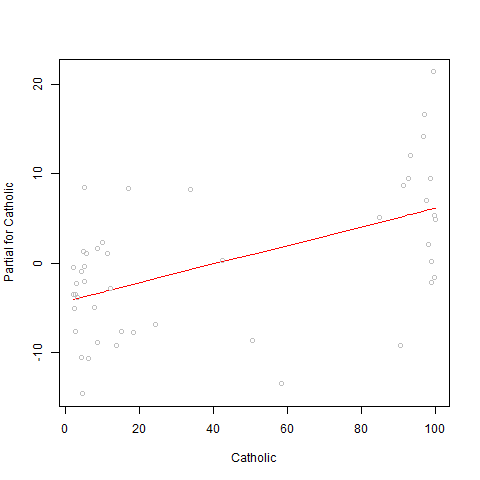
\includegraphics[width=8cm,height=8cm]{catholicSep.png}
	 	\caption[catholicSep]{We see a seperation between catholic regions belows ~30\% and regions above 80\%}
	 	\label{interesting obs}
	 \end{figure}
	 It may be interesting to see if there is any difference between the two types of regions
	 \item
	 Looking at the cheddar dataset, describing the taste of certain cheeses along with several parameters. We look for some outliers.\\
	 
	 We find there is nothing abnormal about the error, and there is only a few high leverages, but the entry that really sticks out is row number 15 due to its high studentized residual and cooks distance.
	 
	 \begin{figure}[H]
	 	\centering
	 	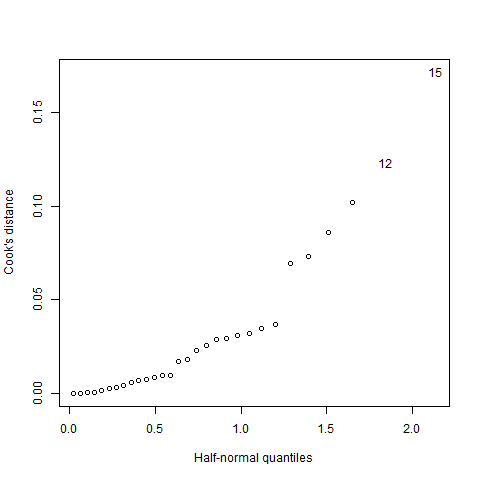
\includegraphics[width=8cm,height=8cm]{cheddarCD.png}
	 	\caption[cheddarCD]{cooks distances from cheddar data}
	 	\label{CD check on teen gamb}
	 \end{figure}
	 
	 a closer look at fifteen reveals 
	 \begin{verbatim}
	 	> cheddar[15,]
	 	taste Acetic   H2S Lactic
	 	15  54.9  6.151 6.752   1.52
	 \end{verbatim}
	 holding a very high taste value, but holding a low lactic value compared to other highly rated cheeses.
	 \\
	 removing it from the model, we see the following performance change.
	 \begin{verbatim}
	 	> cmodel2=lm(taste~.,subset=cooksC<max(cooksC),cheddar)
	 	> summary(cmodel)
	 	
	 	Coefficients:
	 	Estimate Std. Error t value Pr(>|t|)   
	 	(Intercept) -28.8768    19.7354  -1.463  0.15540   
	 	Acetic        0.3277     4.4598   0.073  0.94198   
	 	H2S           3.9118     1.2484   3.133  0.00425 **
	 	Lactic       19.6705     8.6291   2.280  0.03108 * 
	 	
	 	Residual standard error: 10.13 on 26 degrees of freedom
	 	Multiple R-squared:  0.6518,	Adjusted R-squared:  0.6116 
	 	F-statistic: 16.22 on 3 and 26 DF,  p-value: 3.81e-06
	 	
	 	> summary(cmodel2)
	 	
	 	Coefficients:
	 	Estimate Std. Error t value Pr(>|t|)   
	 	(Intercept)  -17.757     17.625  -1.007  0.32335   
	 	Acetic        -2.470      4.004  -0.617  0.54279   
	 	H2S            4.039      1.091   3.702  0.00106 **
	 	Lactic        21.458      7.559   2.839  0.00886 **
	 	
	 	Residual standard error: 8.847 on 25 degrees of freedom
	 	Multiple R-squared:  0.7083,	Adjusted R-squared:  0.6733 
	 	F-statistic: 20.24 on 3 and 25 DF,  p-value: 7.18e-07
	 \end{verbatim}
	 Yet another large jump in r squared values and improved p values, particularly in H2S and lactic, which makes sense due to our previous outliers lactic value.
	 \item
	 The happy data set, looks at how happy students are from the university of chicagos MBA program.
	 \\
	 the normality error assumptions check out, as in we have a seemingly constant variance, normally distributed, without any non linearity.
	 \\
	 looking at the studentized residuals, we notice entry 36 is quite high
	 \begin{verbatim}
	 	> examineStudRes(hmodel)
	 	36          19          16           7          38          37          20          23          35           3 
	 	-3.27601274 -1.67801954 -1.45766638 -1.27738113 -0.99473268 -0.96624585 -0.91144453 -0.89539011 -0.87176009 -0.57454041 ...
	 \end{verbatim}
	 with the accompanying diagram
	 \begin{figure}[H]
	 	\centering
	 	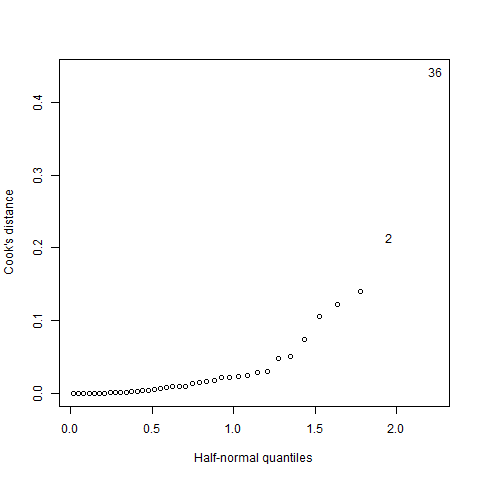
\includegraphics[width=8cm,height=8cm]{happyCD.png}
	 	\caption[happyCD]{cooks distances from happy data set}
	 	\label{CD check on happy data set}
	 \end{figure}
	 we see that entry 36 is looking like quite the outlier, looking deeper.
	 \begin{verbatim}
	 	> happy[36,]
	 	happy money sex love work
	 	36     2     0   0    2    2
	 \end{verbatim}
	 very clear outlier here. There is some incorrect data input as it claims a household family income of 0 dollars. This could be an indication that they have no family, but for now it is too extreme. Removing the point and comparing models we get...
	 \begin{verbatim}
	 	Call:
	 	lm(formula = happy ~ ., data = happy)
	 	Coefficients:
	 	Estimate Std. Error t value Pr(>|t|)    
	 	(Intercept) -0.072081   0.852543  -0.085   0.9331    
	 	money        0.009578   0.005213   1.837   0.0749 .  
	 	sex         -0.149008   0.418525  -0.356   0.7240    
	 	love         1.919279   0.295451   6.496 1.97e-07 ***
	 	work         0.476079   0.199389   2.388   0.0227 *  
	 	
	 	Residual standard error: 1.058 on 34 degrees of freedom
	 	Multiple R-squared:  0.7102,	Adjusted R-squared:  0.6761 
	 	F-statistic: 20.83 on 4 and 34 DF,  p-value: 9.364e-09
	 	
	 	> summary(hmodel2)
	 	
	 	Call:
	 	lm(formula = happy ~ ., data = happy, subset = cooksH < max(cooksH))
	 	Coefficients:
	 	Estimate Std. Error t value Pr(>|t|)    
	 	(Intercept)  0.920460   0.810476   1.136    0.264    
	 	money        0.006680   0.004681   1.427    0.163    
	 	sex         -0.487967   0.383259  -1.273    0.212    
	 	love         1.953712   0.260722   7.493 1.29e-08 ***
	 	work         0.305096   0.183392   1.664    0.106    
	 	
	 	Residual standard error: 0.9332 on 33 degrees of freedom
	 	Multiple R-squared:  0.7347,	Adjusted R-squared:  0.7026 
	 	F-statistic: 22.85 on 4 and 33 DF,  p-value: 4.064e-09
	 \end{verbatim}
	 we see a minor increase in R squared values, and major improvements in p values except for money, which interestingly, went up after removing the term. This also made work no longer a powerful predictor.
\end{enumerate}
\end{document}
